\subsection{推理阶段性能剖析}\label{sec:inference}

本节专门分析 SO-101 在线控制循环中的 ACT 推理阶段。
这里的“推理阶段”并不只是一次 \texttt{ACT.forward()}，
而是从 \texttt{predict\_action()} 收到 observation 开始，
经过动作缓存判断、必要时的观测预处理、ACT 模型前向、动作队列写入、
再到动作反归一化返回的完整路径。

当前实验配置中，ACT 的 \texttt{chunk\_size} 与
\texttt{n\_action\_steps} 均为 100，单次完整模型推理输出
\((B,\texttt{chunk\_size},\texttt{action\_dim})=(1,100,6)\) 的动作序列。
因此在线循环的大多数帧并不会重新执行模型前向，而是直接从
\texttt{\_action\_queue} 中取出上一次推理缓存的下一帧动作。
这一区别是理解第~\ref{sec:inference} 节所有时间数据的前提：
\texttt{chunk\_size} 主要是在时间上分摊单次 ACT 前向开销，
而不是让一次 ACT 前向本身变快。

\subsubsection{\texttt{select\_action} 与动作队列}

LeRobot 在 \texttt{predict\_action()} 外层先检查策略对象的动作队列。
如果 \texttt{\_action\_queue} 非空，主循环直接
\texttt{popleft()} 取出缓存动作，再通过 \texttt{postprocessor}
反归一化为真实舵机目标；这一帧会跳过图像 tensor 转换、
\texttt{preprocessor} 和 \texttt{ACT.forward()}。
只有当队列为空时，系统才会走完整推理路径：
把 numpy observation 转为 PyTorch Tensor，执行归一化预处理，
调用 \texttt{policy.select\_action()}，继而触发
\texttt{predict\_action\_chunk()} 和 \texttt{ACT.forward()}。
模型一次产生 100 帧归一化动作，写入队列后立即弹出第 0 帧返回；
后续 99 帧由队列快速路径逐帧取用。

\begin{figure}[htbp]
  \centering
  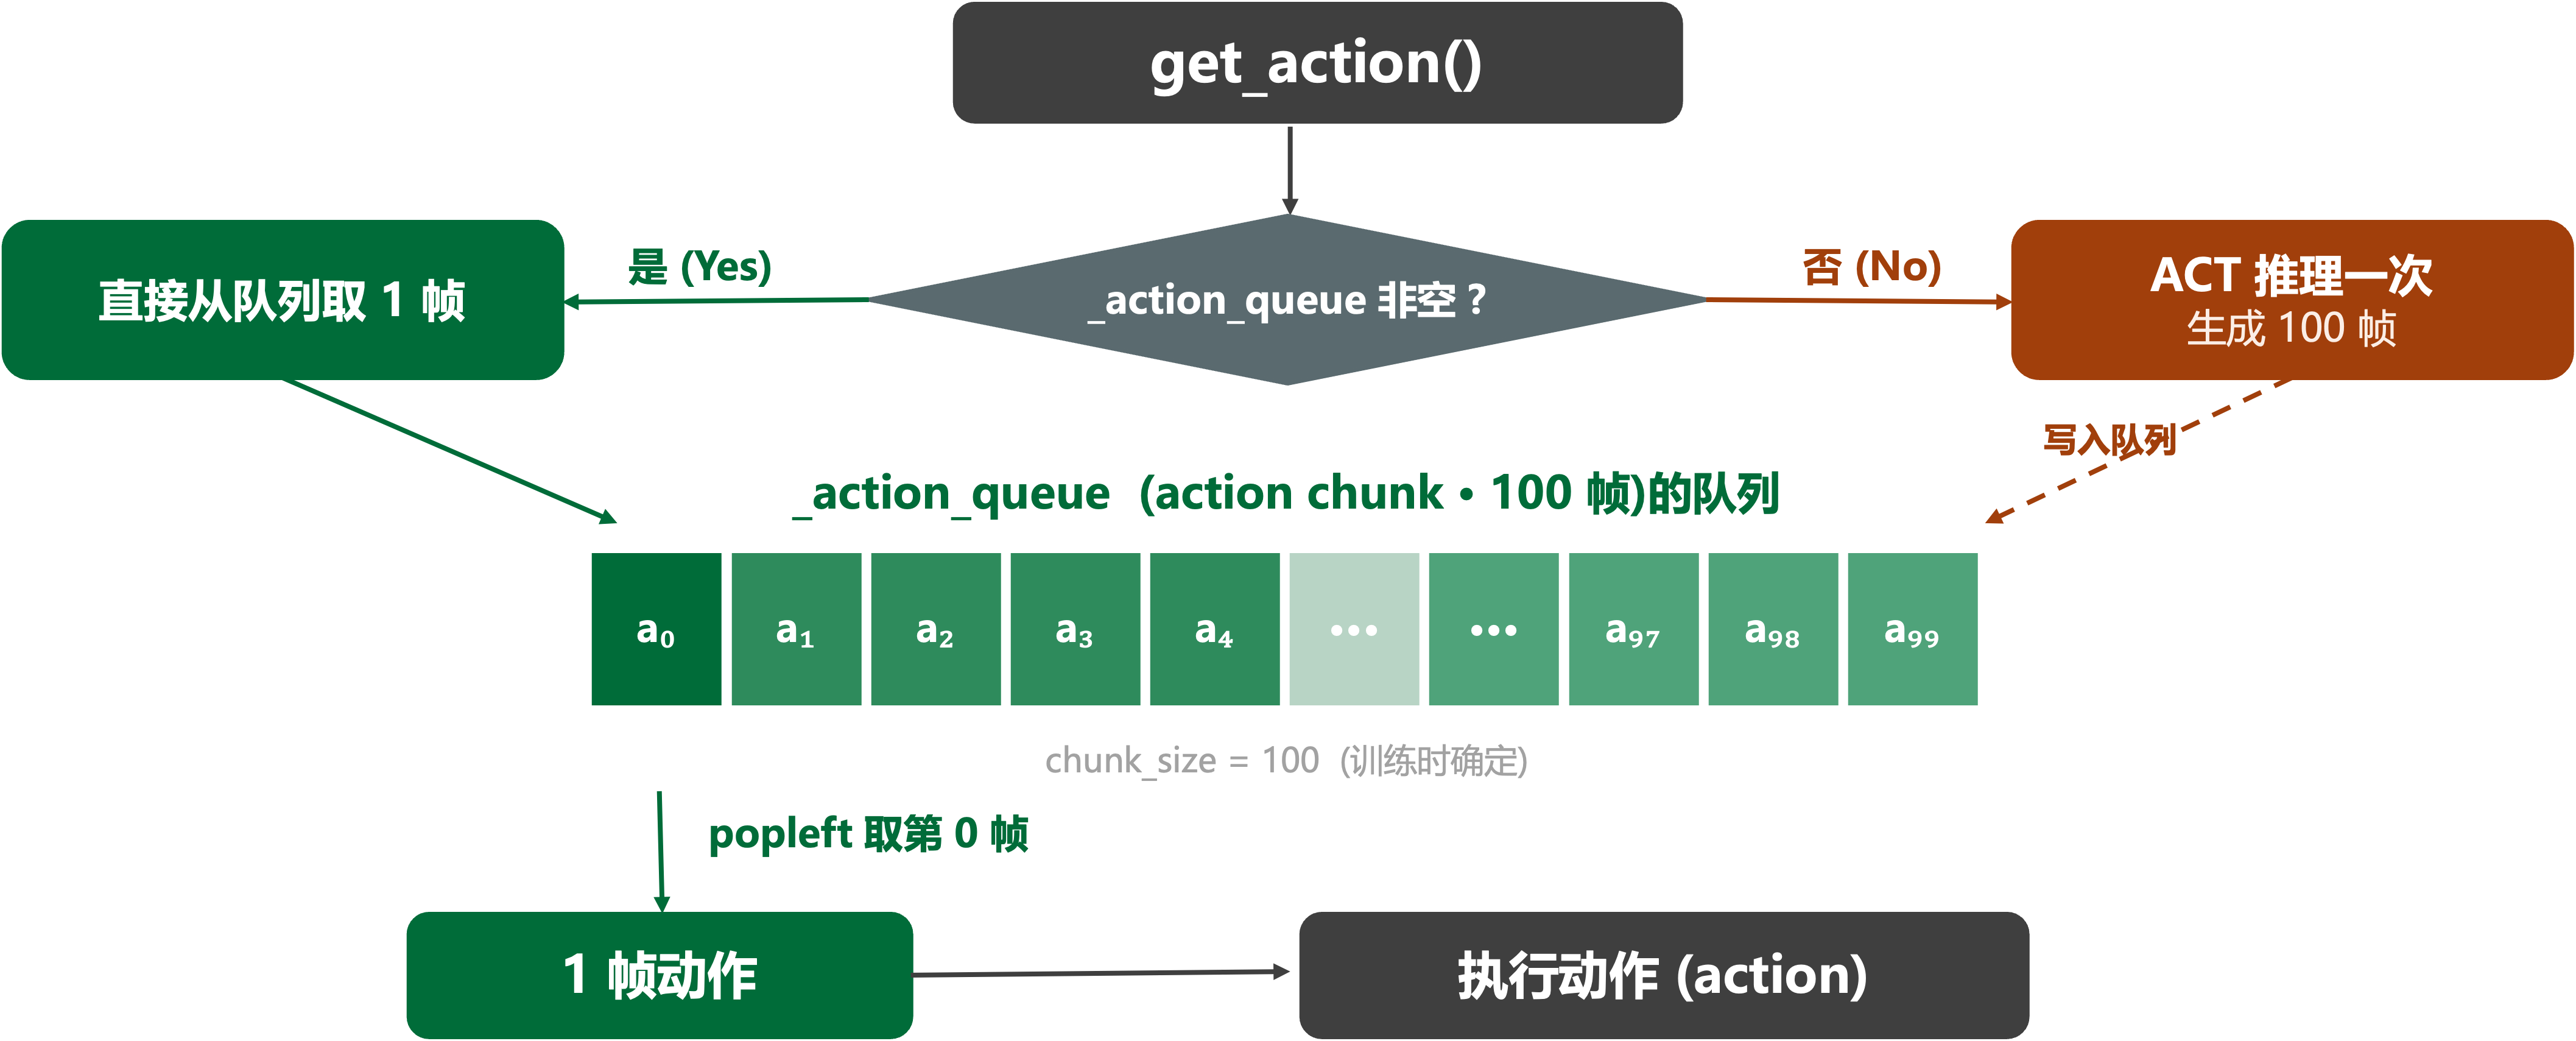
\includegraphics[width=\textwidth]{3_性能分析/image/act_select_action_queue.png}
  \caption{ACT 在线推理中动作队列快速路径与完整推理路径}
  \label{fig:act-select-action-queue}
\end{figure}

图~\ref{fig:act-select-action-queue} 说明了
\texttt{chunk\_size=100} 下的两种时间尺度：
队列非空帧只承担动作取队列和反归一化，属于轻量路径；
队列为空帧才承担完整 ACT 前向，属于重推理路径。
因此，按 episode 统计得到的 inference 占比，本质上是少数重推理帧
在 100 帧执行周期内被均摊后的结果。

\subsubsection{一次完整 ACT 推理的数据流}

队列为空时，\texttt{predict\_action()} 会先把原始 observation
整理成 ACT 可接受的 batch。两路相机图像从
\((H,W,C)\) 的 \texttt{uint8} numpy 数组转换为
\((1,3,360,640)\) 的 \texttt{float32} Tensor；
关节状态从 \((6,)\) 转为 \((1,6)\)。
随后 \texttt{preprocessor} 使用随 checkpoint 保存的训练集
mean/std 对图像、state 进行归一化。进入 \texttt{ACT.forward()}
后，推理态下不运行训练用 VAE encoder，而是使用全零 latent。

\begin{figure}[htbp]
  \centering
  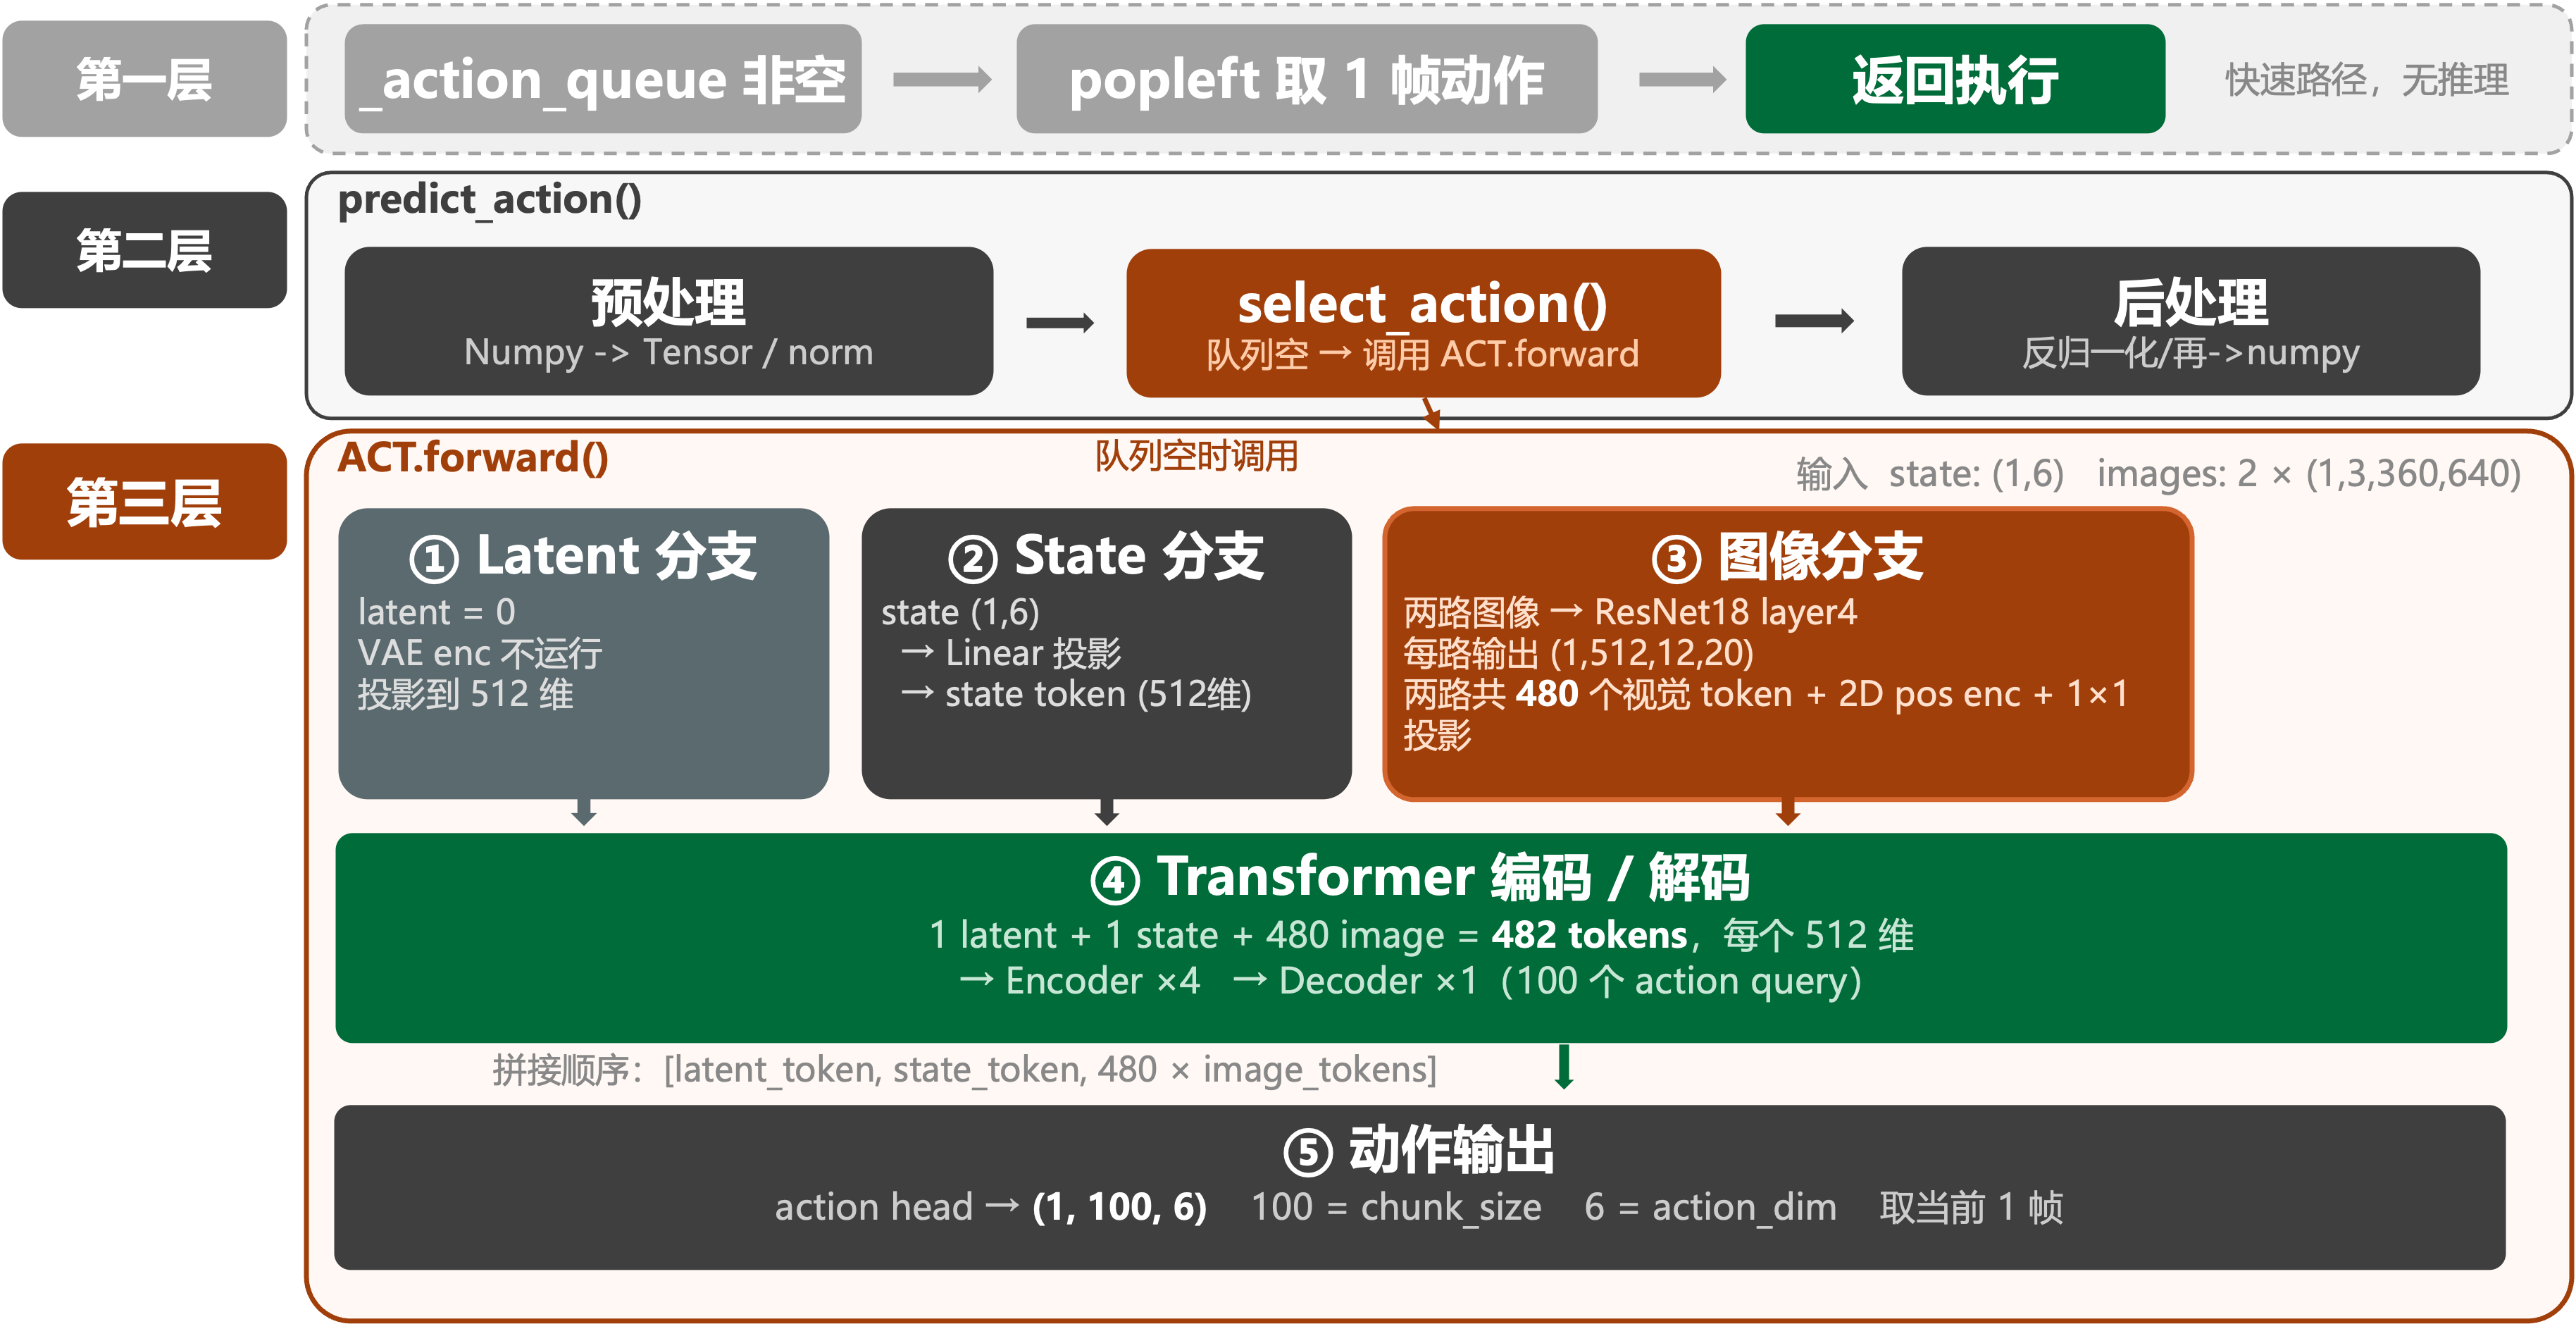
\includegraphics[width=\textwidth]{3_性能分析/image/act_forward_dataflow.png}
  \caption{队列为空时一次完整 ACT 推理的数据流与模型结构}
  \label{fig:act-forward-dataflow}
\end{figure}

图~\ref{fig:act-forward-dataflow} 中，视觉分支是主要计算来源。
每路 \(640\times360\) 图像经 ResNet18 的 \texttt{layer4}
得到 \(512\times12\times20\) 特征图，两路相机共形成
480 个视觉 token；再加上 1 个 state token 和 1 个全零 latent token，
构成长度 482、维度 512 的 Transformer Encoder 输入序列。
Decoder 使用 100 个可学习 query，最终通过线性层输出
100 帧、每帧 6 维的归一化动作。

\subsubsection{时间剖析：\texttt{chunk\_size} 参数扫描}

实验 01 在树莓派 5 上对同一 ACT 抓取瓶子策略扫描 \texttt{chunk\_size}，
取值覆盖 $\{1, 3, 5, 10, 20, 50, 100\}$，每个取值固定记录 20 个 episode，
其它参数（模型权重、分辨率、目标 fps）保持一致。
原始数据与绘图脚本保存在 \src{实验 01：chunk\_size 参数扫描}。
后文先看四个阶段的时间占比如何随 \texttt{chunk\_size} 变化，
再单独看 FPS 的增长曲线，最后用代表性数值表汇总。

\paragraph{阶段时间占比随 \texttt{chunk\_size} 的演化}
图~\ref{fig:chunk-size-time-pct} 给出了 Observation/Inference/Execution/Wait
（\texttt{obs}/\texttt{inference}/\texttt{action}/\texttt{wait}）四阶段
平均占比（20 episode 均值）随 \texttt{chunk\_size} 的变化曲线。
\texttt{inference\_pct} 从 cs=1 时的 97.6\% 单调下降到 cs=100 时的 36.5\%，
对应 \texttt{wait\_pct} 从 0\% 单调上升到 43.3\%；
\texttt{obs\_pct} 从近 0\% 缓慢增长到 15.4\%，
\texttt{action\_pct} 始终保持在 5\% 以内。
这条主曲线说明 \texttt{chunk\_size} 越大，
单帧分摊到的推理工作量就越小，控制循环把更多预算还给 \texttt{wait}
（即在帧内等待 fps 节拍），推理不再压满整个 33.3 ms 时间预算。
观测和执行阶段的占比上升只是相对结果——
其绝对耗时基本恒定，只是因为 inference 缩短才在比例上变得显眼。

\begin{figure}[htbp]
  \centering
  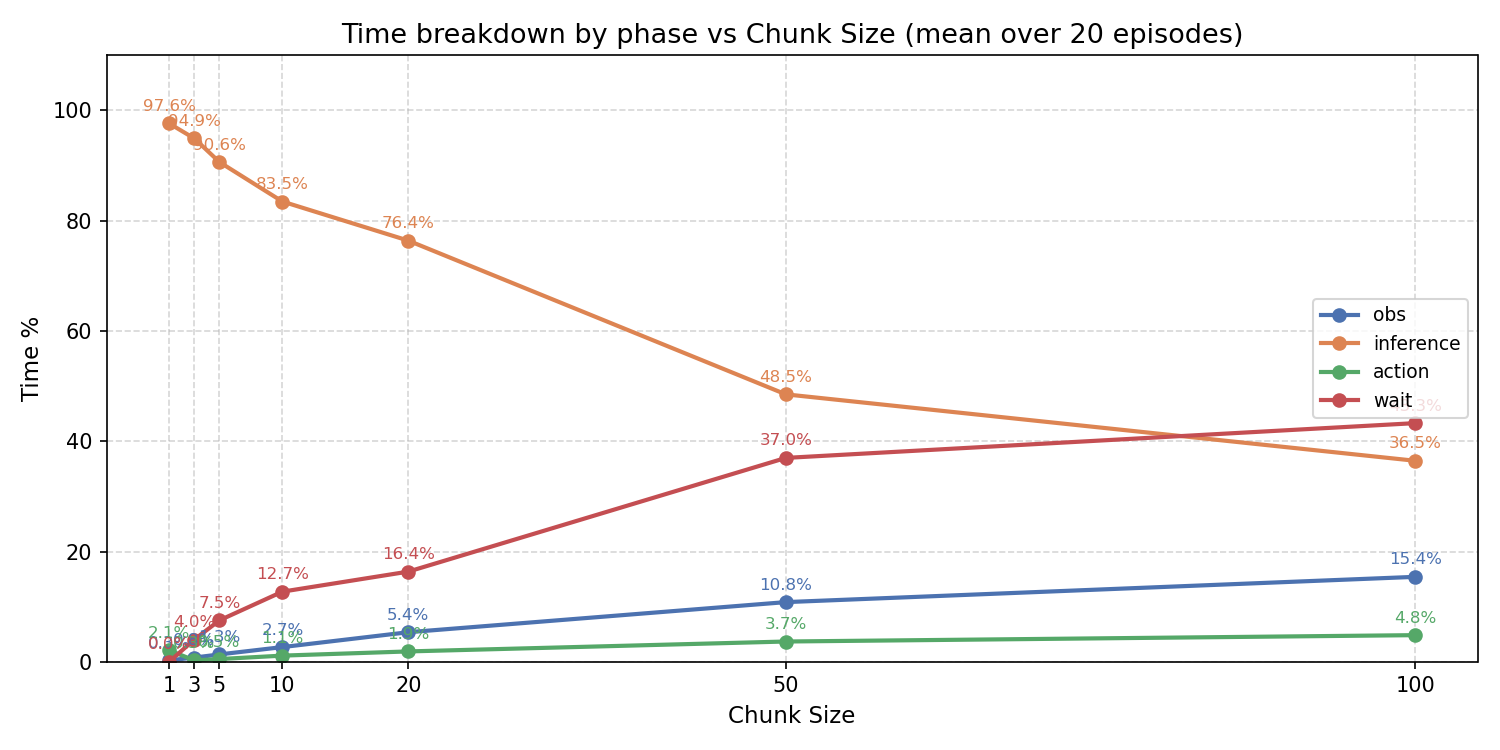
\includegraphics[width=\textwidth]{../实验/01_chunk_size参数扫描/chart1_time_pct.png}
  \caption{\texttt{chunk\_size} 对控制循环阶段时间占比的影响}
  \label{fig:chunk-size-time-pct}
\end{figure}

\paragraph{FPS 随 \texttt{chunk\_size} 的非线性增益}
图~\ref{fig:chunk-size-fps} 给出了实测平均 FPS 随 \texttt{chunk\_size} 的变化曲线。
FPS 从 cs=1 的 0.8 上升到 cs=100 的 18.7，但增长曲线高度非线性：
cs=1$\to$10 时 FPS 提升约 6.6 倍（0.8$\to$5.3），cs=10$\to$50 时再提升约 2.9 倍，
而 cs=50$\to$100 时增益仅约 1.2 倍（15.4$\to$18.7），呈现典型的边际递减。
原因是单次完整 ACT 推理的绝对耗时接近恒定（约 1.5--2.0\,s/次，均值约 1.9\,s），
分块机制只是把这一次重推理在时间上摊薄到更多控制帧上，
而不是降低 \texttt{ACT.forward()} 本身的计算量；
当 cs 增大到推理被摊薄到接近 fps 目标时，
等待阶段就成为主循环新的瓶颈，进一步增大 cs 不再带来等比增益。

\begin{figure}[htbp]
  \centering
  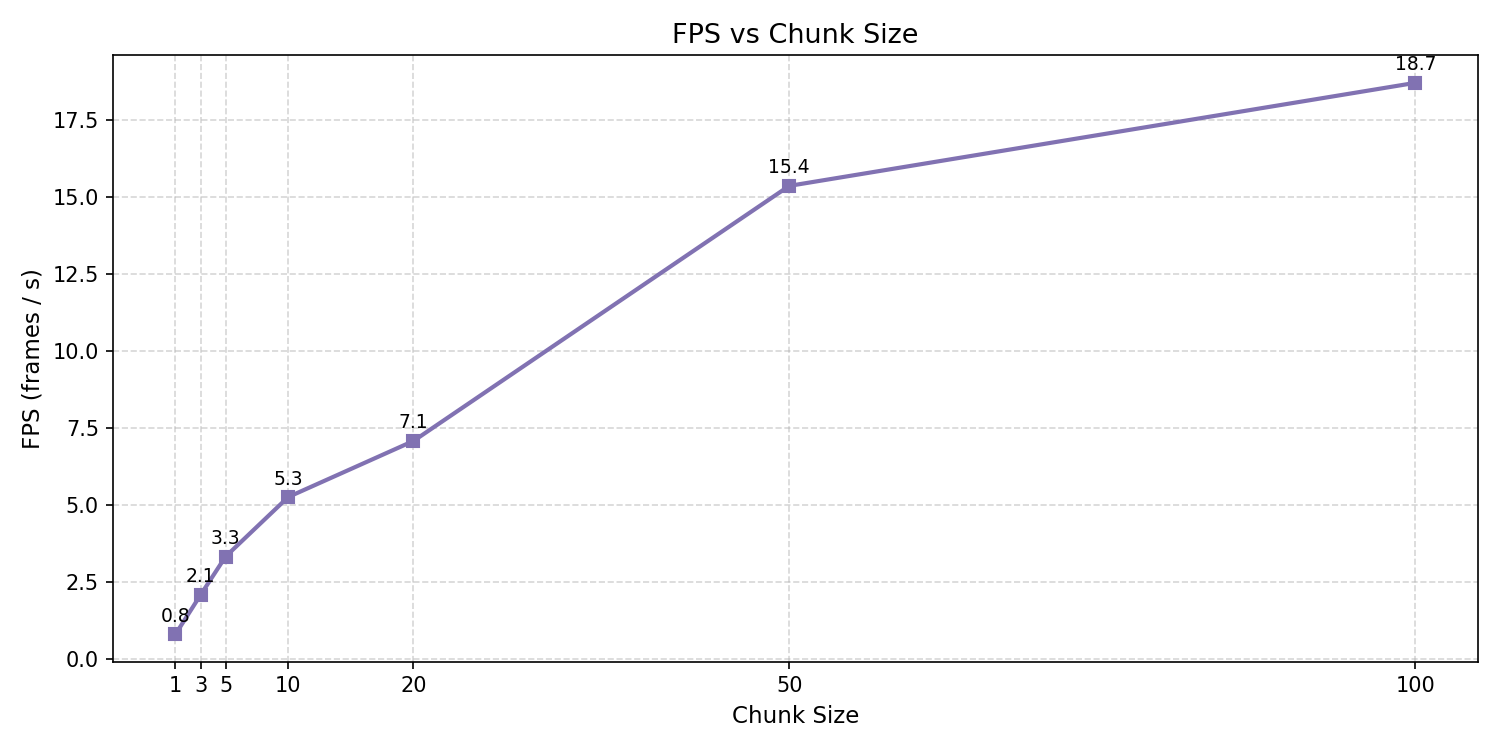
\includegraphics[width=0.92\textwidth]{../实验/01_chunk_size参数扫描/chart2_fps.png}
  \caption{\texttt{chunk\_size} 对控制循环 FPS 的影响}
  \label{fig:chunk-size-fps}
\end{figure}


cs=100 在树莓派 5 上能跑到 $\approx$18.7 fps，距 30 fps 目标仍有约 38\% 缺口；
而此时 \texttt{wait\_pct} 已升至 43.3\%，
说明继续增大 cs 已经不能进一步把 fps 推到 30——
要逼近目标必须从减小单次推理绝对耗时入手，
也就是后文（第~\ref{ch:opt} 章）讨论的优化方向。

\subsubsection{单次 ACT 推理耗时分解}\label{sec:act-infer-breakdown}

上面的 episode 级统计能够说明 \texttt{chunk\_size} 如何分摊推理开销，
但还不能回答”一次完整 ACT 推理内部究竟慢在哪里”。
实验在 \texttt{modeling\_act.py} 的 \texttt{select\_action()} 和 \texttt{ACT.forward()} 内
插入计时点，通过环境变量 \texttt{LEROBOT\_PROFILING=1} 启用，数据直接写入 CSV。
在树莓派 5 上记录了 6 次队列为空的完整推理，结果汇总于表~\ref{tab:act-single-infer-profile}。

\begin{table}[htbp]
\centering
\small
\begin{tabular}{lrrr}
  \toprule
  模块 & 平均耗时 ms & 标准差 ms & 占完整推理比例 \\
  \midrule
  \texttt{select\_action} 完整路径 & 1924.8 & 414.9 & 100.0\% \\
  \quad ResNet18 + 投影 & 1281.1 & 259.9 & 66.6\% \\
  \quad Transformer Encoder & 569.5 & 506.3 & 29.6\% \\
  \quad Transformer Decoder & 44.0 & 4.4 & 2.3\% \\
  \quad action\_head & 0.7 & 0.8 & $<$0.1\% \\
  队列非空快速路径（对照） & $<$1 ms & — & — \\
  \bottomrule
\end{tabular}
\caption{ACT 单次完整推理（队列为空时）的逐模块耗时分解}
\label{tab:act-single-infer-profile}
\end{table}

图~\ref{fig:act-infer-breakdown} 给出了各模块的耗时柱状图。

\begin{figure}[htbp]
  \centering
  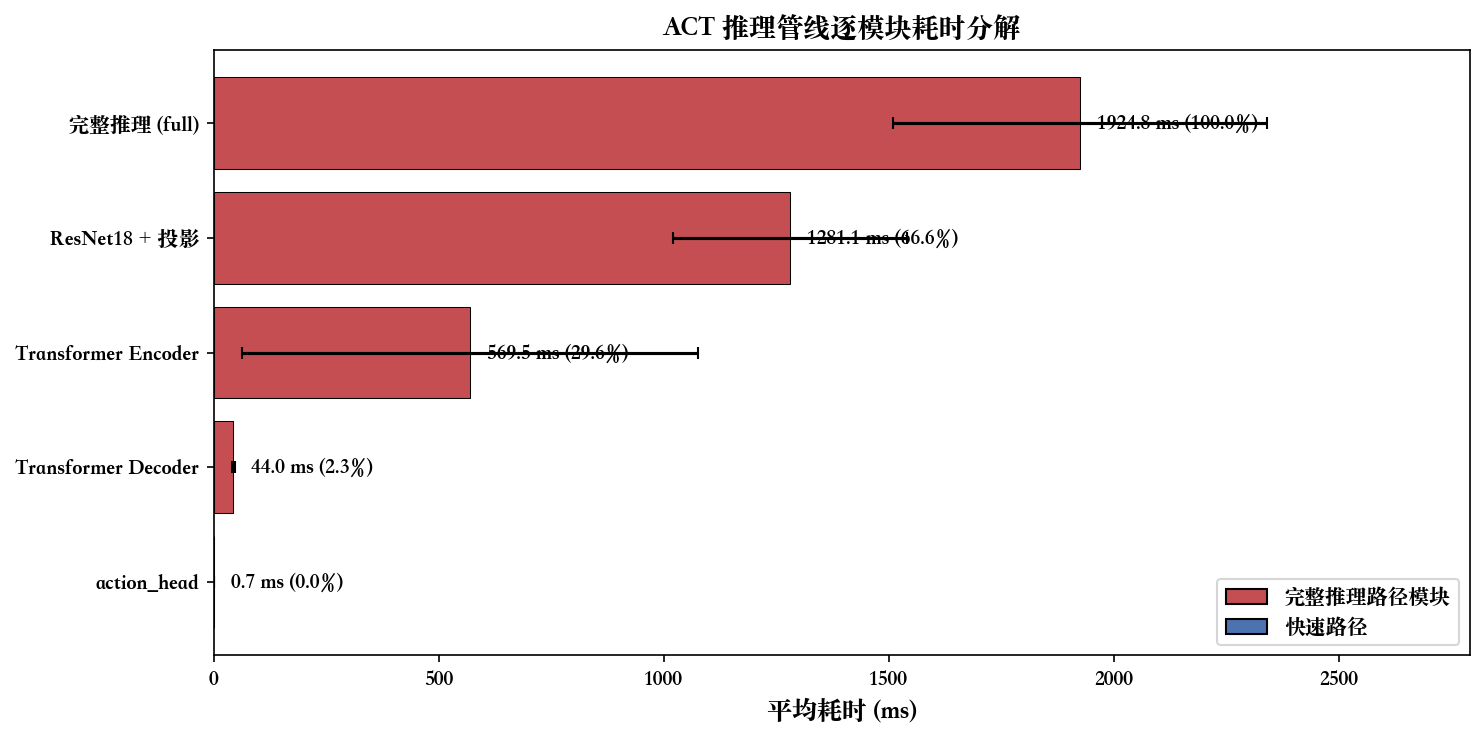
\includegraphics[width=\textwidth]{3_性能分析/image/inference_breakdown.png}
  \caption{ACT 推理管线逐模块耗时分解}
  \label{fig:act-infer-breakdown}
\end{figure}

\textbf{关键发现}：ResNet18 视觉特征提取（两路 ResNet18 backbone + 位置编码 + 1×1 投影）
占据完整推理时间的 \textbf{66.6\%}（平均 1281 ms），是第一瓶颈。
Transformer Encoder 次之，占 29.6\%（569 ms）。
Decoder 和 action\_head 占比极低（2.3\% 和 $<$0.1\%），
不是优化重点。
队列非空快速路径耗时不足 1 ms，与后处理相当，
验证了动作缓存机制的有效性。

\subsubsection{PyTorch 线程行为与推理优化研究现状}\label{sec:thread-behavior}

PyTorch 在 ARM CPU 上使用 OpenMP 并行框架，通过 ATen 线程池调度矩阵运算。
系统调用追踪显示 futex 调用共计 64,569 次 / 40 s episode，
其中 27 线程并行累计等待时间达 3,252 s，
说明多线程同步开销在 ARM CPU 上不可忽略。

推理优化方向（如 INT8 量化、算子融合、线程亲和性、NEON SIMD 加速等）
已有大量文献研究，此处不再展开。
